% TikZ diagram: Physical Classroom to Digital Game Mapping
% Compile with: pdflatex physical-to-digital-mapping.tex

\documentclass[tikz,border=10pt]{standalone}
\usepackage{tikz}
\usetikzlibrary{shapes,arrows,positioning,fit,backgrounds}

\begin{document}
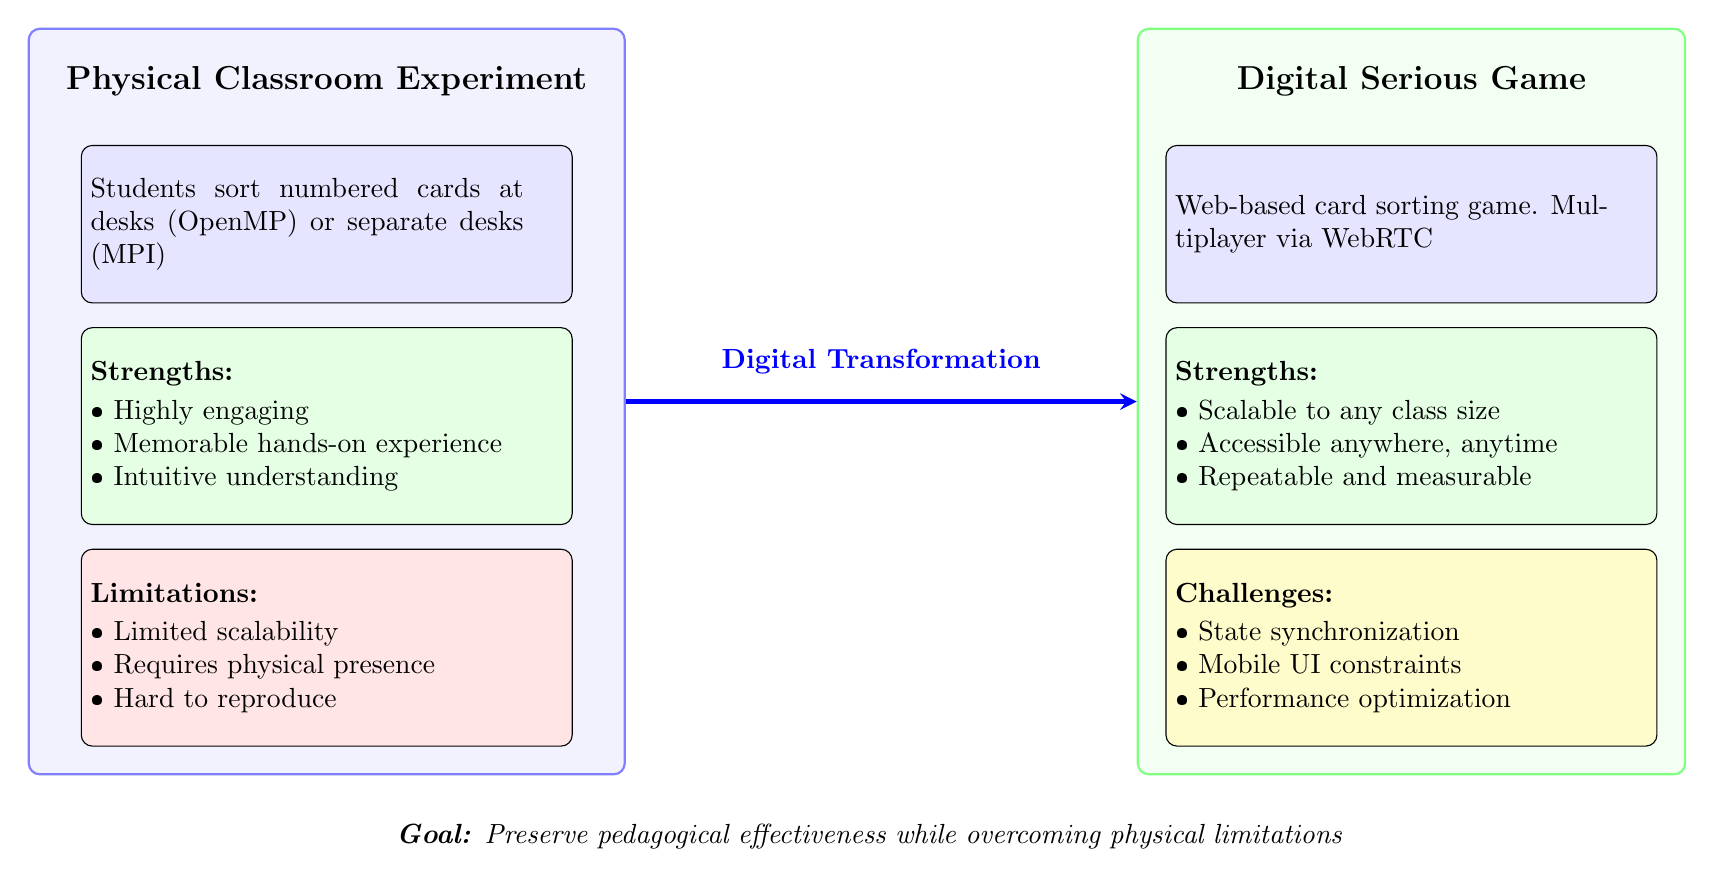
\begin{tikzpicture}[
        node distance=1.5cm,
        box/.style={rectangle, draw, fill=blue!10, text width=6cm, align=justify, minimum height=1.2cm, rounded corners},
        arrow/.style={->, >=stealth, thick},
        label/.style={font=\bfseries\large}
    ]

    % Physical Experiment Side (LEFT)
    \node[label] (physical-label) {Physical Classroom Experiment};
    \node[box, below=0.5cm of physical-label, minimum height=2cm] (physical-desc) {
        \begin{minipage}{5.5cm}
        Students sort numbered cards at desks (OpenMP) or separate desks (MPI)
        \end{minipage}
    };

    \node[box, below=0.3cm of physical-desc, fill=green!10, minimum height=2.5cm] (physical-pros) {
        \begin{minipage}{5.5cm}
        \textbf{Strengths:}\\[2pt]
        • Highly engaging\\
        • Memorable hands-on experience\\
        • Intuitive understanding
        \end{minipage}
    };

    \node[box, below=0.3cm of physical-pros, fill=red!10, minimum height=2.5cm] (physical-cons) {
        \begin{minipage}{5.5cm}
        \textbf{Limitations:}\\[2pt]
        • Limited scalability\\
        • Requires physical presence\\
        • Hard to reproduce
        \end{minipage}
    };

    % Digital Game Side (RIGHT) - positioned relative to left side
    \node[label, right=8cm of physical-label] (digital-label) {Digital Serious Game};
    \node[box, below=0.5cm of digital-label, minimum height=2cm] (digital-desc) {
        \begin{minipage}{5.5cm}
        Web-based card sorting game. Multiplayer via WebRTC
        \end{minipage}
    };

    \node[box, below=0.3cm of digital-desc, fill=green!10, minimum height=2.5cm] (digital-pros) {
        \begin{minipage}{5.5cm}
        \textbf{Strengths:}\\[2pt]
        • Scalable to any class size\\
        • Accessible anywhere, anytime\\
        • Repeatable and measurable
        \end{minipage}
    };

    \node[box, below=0.3cm of digital-pros, fill=yellow!20, minimum height=2.5cm] (digital-challenge) {
        \begin{minipage}{5.5cm}
        \textbf{Challenges:}\\[2pt]
        • State synchronization\\
        • Mobile UI constraints\\
        • Performance optimization
        \end{minipage}
    };

    % Background boxes - give them names so we can reference them for the arrow
    \begin{scope}[on background layer]
        \node[fit=(physical-label)(physical-desc)(physical-pros)(physical-cons),
            fill=blue!5, draw=blue!50, thick, rounded corners, inner sep=10pt] (physical-box) {};
        \node[fit=(digital-label)(digital-desc)(digital-pros)(digital-challenge),
            fill=green!5, draw=green!50, thick, rounded corners, inner sep=10pt] (digital-box) {};
    \end{scope}

    % Goal - centered between both BACKGROUND boxes, positioned BELOW them
    \path (physical-box.south) -- (digital-box.south) coordinate[midway] (boxes-bottom-mid);
    \node[below=0.5cm of boxes-bottom-mid, font=\itshape, text width=14cm, align=center] (goal) {
        \textbf{Goal:} Preserve pedagogical effectiveness while overcoming physical limitations
    };

    % Arrow in the middle - connecting the two background boxes
    \draw[arrow, ultra thick, blue] (physical-box.east) -- node[above, font=\bfseries, yshift=2mm] {Digital Transformation} (digital-box.west);

\end{tikzpicture}
\end{document}
